\documentclass[tikz,border=1mm,10pt,dvipsnames]{standalone}
\usetikzlibrary{backgrounds}

%\usetikzlibrary{shapes.misc}
%\tikzset{cross/.style={cross out, draw=black, minimum size=2*(#1-\pgflinewidth), inner sep=0pt, outer sep=0pt},
%%default radius will be 1pt.
%cross/.default={1pt}}

\begin{document}
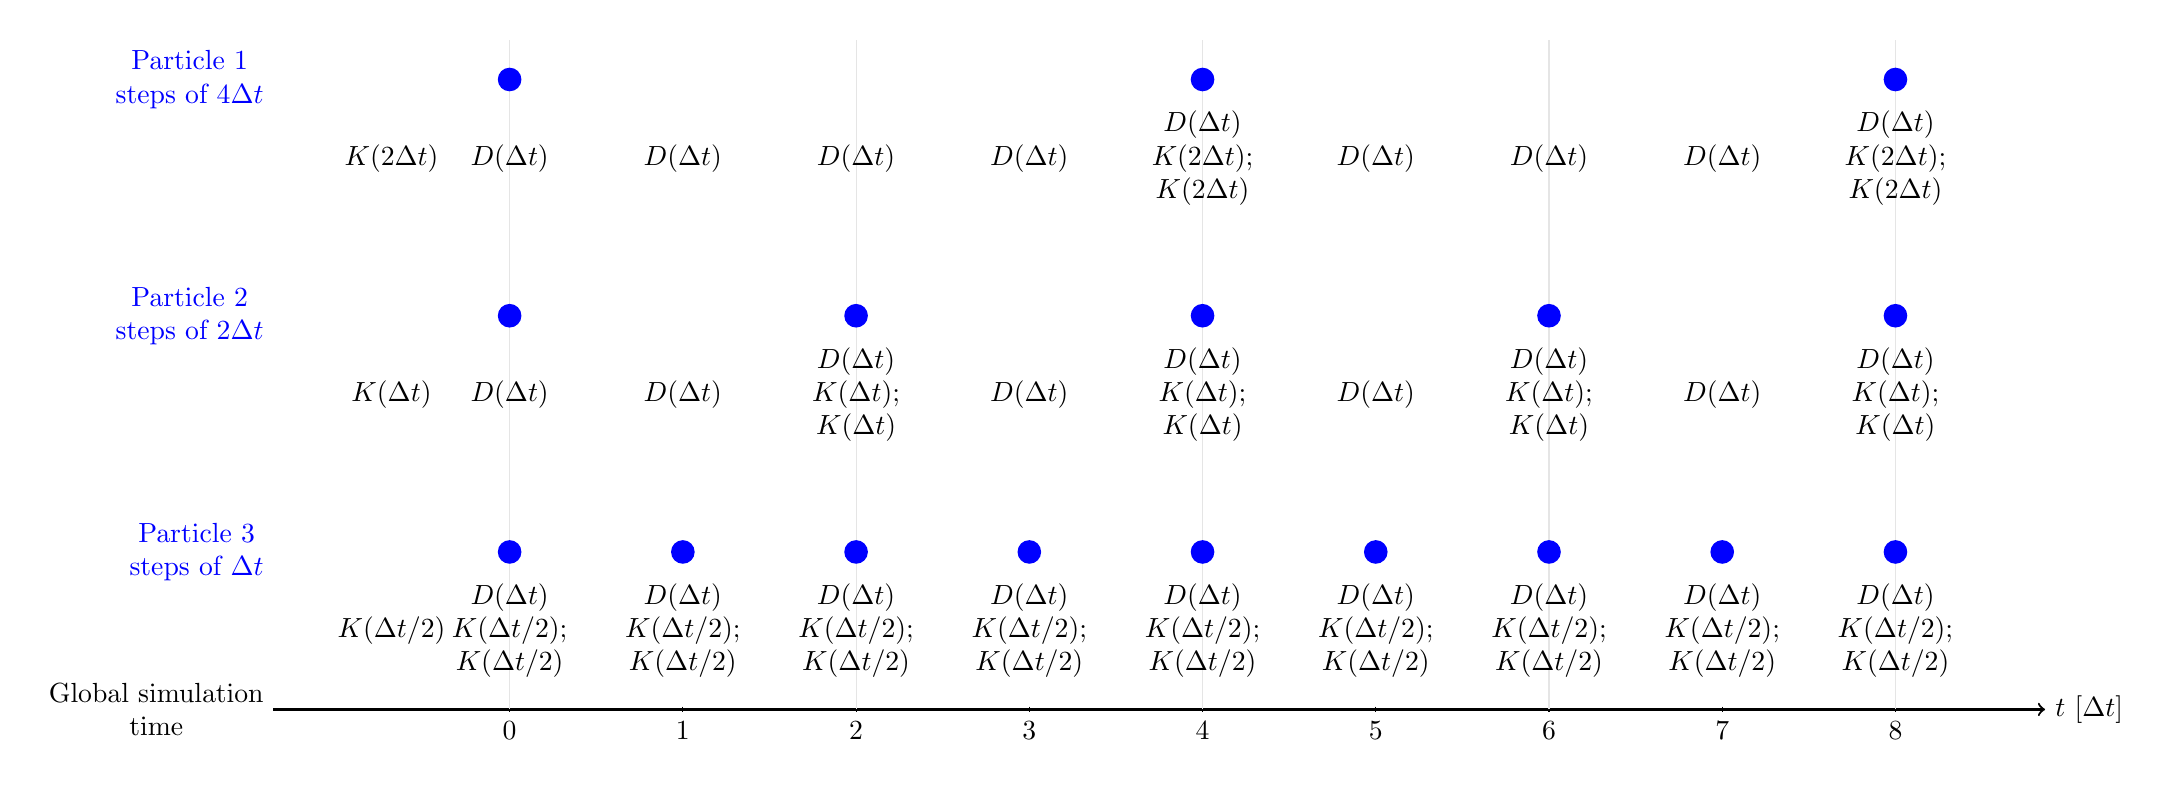
\begin{tikzpicture}[transform shape, background rectangle/.style={fill=white}, show background rectangle]

	\def\hydroColor{blue};
	\def\rtColor{ForestGreen};

	\def\Xzero{-3cm};
	\def\Xmax{19.5cm};
	\def\Yzero{0cm};
	\def\Ymax{8.5cm};
	\def\partoneY{8cm};
	\def\parttwoY{5cm};
	\def\partthreeY{2cm};
	\def\radius{0.15cm};
	\def\dy{1cm}
	\def\dx{2.2cm}


	% X Axis
	\draw[thick, ->] (\Xzero,\Yzero) -- (\Xmax,\Yzero) node[anchor=west] {$t$ [$\Delta t]$};
	\foreach \x in {0,1,2,3,4,5,6,7,8}
		\draw (\x * \dx, 1pt) -- (\x * \dx,-1pt) node[anchor=north] {$\x$};

	% Y Axis
%	\draw[thick] (-1,0) -- (-1,8.5); %node[anchor=south east] {y axis};
	% Axes ticks
%	\foreach \y in {0,1,2,3,4,5,6,7,8}
%		\draw (\Xzero-1pt,\y cm) -- (\Xzero-1pt,\y cm) node[anchor=east] {$\y$};


	\foreach \x in {0, 2, 4, 6, 8}
		\draw [color=gray!20] (\x * \dx, \Yzero) -- (\x * \dx, \Ymax);


	% Particle labels
	\draw node[anchor=east, align=center, \hydroColor] at (\Xzero, \partoneY) {Particle 1\\ steps of $4 \Delta t$};

	\draw node[anchor=east, align=center, \hydroColor] at (\Xzero, \parttwoY) {Particle 2\\ steps of $2 \Delta t$};

	\draw node[anchor=east, align=center, \hydroColor] at (\Xzero, \partthreeY) {Particle 3\\ steps of $\Delta t$};

	\draw node[anchor=east, align=center, black] at (\Xzero, \Yzero) {Global simulation\\time};


	% Particle 1 Hydro Activity
	\foreach \px in {0, 4, 8}
		\fill[color=\hydroColor] (\px * \dx,\partoneY) circle (\radius);


	% Particle 2 Hydro Activity
	\foreach \px in {0, 2, 4, 6, 8}
		\fill[color=\hydroColor] (\px * \dx,\parttwoY) circle (\radius);


	% Particle 3 Hydro Activity
	\foreach \px in {0, 1, 2, 3, 4, 5, 6, 7, 8}
		\fill[color=\hydroColor] (\px * \dx,\partthreeY) circle (\radius);


	% Particle 1 operators
	\node at (\Xzero + 1.5cm, \partoneY - \dy) {$K(2 \Delta t)$};
	\foreach \px in {0, 1, 2, 3, 5, 6, 7}
		\node at (\px * \dx, \partoneY - \dy) {$D(\Delta t)$};

	\foreach \px in {4, 8}
		\node[align=center] at (\px * \dx, \partoneY - \dy)
			{$D(\Delta t) $\\$ K(2 \Delta t)$;\\ $K(2 \Delta t)$};

	% Particle 2 operators
	\node at (\Xzero + 1.5cm, \parttwoY - \dy) {$K(\Delta t)$};
	\foreach \px in {0, 1, 3, 5, 7}
		\node at (\px * \dx, \parttwoY - \dy) {$D(\Delta t)$};
	\foreach \px in {2, 4, 6, 8}
		\node[align=center] at (\px * \dx, \parttwoY - \dy)
			{$D(\Delta t) $\\$ K( \Delta t)$;\\ $K(\Delta t)$};


	% Particle 3 operators
	\node at (\Xzero + 1.5cm, \partthreeY - \dy) {$K(\Delta t / 2)$};
	\foreach \px in {0, 1, 2, 3, 4, 5, 6, 7, 8}
		\node[align=center] at (\px * \dx, \partthreeY - \dy)
			{$D(\Delta t) $\\$ K( \Delta t/2)$;\\ $K(\Delta t/2)$};


\end{tikzpicture}
\end{document}